\chapter{Motores de reglas}
De forma general, un motor de reglas es una herramienta de software que permite la ejecución de reglas de negocio. Es decir, permite la evaluación de expresiones y la opcional ejecución de acciones y/o retorno de valores, en función de los resultados de la evaluación de expresiones.

Es también de uso común el término Sistema de Gestión de Reglas de Negocio, que a las capacidades mencionadas anteriormente le suma capacidades para la gestión de reglas. En este trabajo, en pos de la brevedad, se utilizarán los términos de forma intercambiable.

\section{Criterio de Evaluación.}
Existen varios proyectos que cuentan con las capacidades descritas en la sección anterior. A continuación, se presentan las características que serán utilizadas para la comparación entre los mismos.

\paragraph{Gestión de las reglas.}
¿Brinda el proyecto herramientas o mecanismos para tareas de la gestión de las reglas, como la creación, modificación, eliminación, evaluación y versionado?

Estas capacidades son necesarias para cumplir con los objetivos de este trabajo, teniendo que ser implementadas en caso de no ser ofrecidas por la herramienta en cuestión.

\paragraph{Integración.}
¿Cómo puede ser el motor integrado con el sistema actual? ¿Cómo se realiza el intercambio de información entre el motor de reglas y el sistema? ¿Cuenta el motor con documentación relevante y actualizada?

Restricciones en los formatos de intercambio de información entre el \acrshort{si} y el motor de reglas imponen también restricciones a la hora de realizar la integración.
Documentación insuficiente o desactualizada resulta en un mayor tiempo requerido y propensidad a errores, siendo lo contrario cierto para documentación completa y actualizada.

\paragraph{Mantenimiento.}
¿Cuenta el proyecto con mantenedores activos? ¿Existen bugs o incompatibilidades que puedan afectar a este trabajo?

\paragraph{Expresividad.}
¿Con qué lenguaje o lenguajes permite el motor la expresión de las reglas? El o los lenguajes deben tener la expresividad suficiente para los cálculos referentes a las cuotas de la obra social.

En concordancia con los objetivos planteados, se prefieren lenguajes que sean inteligibles para personal sin conocimientos específicos de programación.

En pos de facilitar la comparación de los distintos motores, se proveerán ejemplos de reglas que provean funcionalidad correspondiente al código escrito en Java en \cref{lst:calculo_referencia} \cref{lst:interfaz_servicio} y \cref{lst:clase_afiliación}.

\begin{listing}[H]
	\caption{Cálculo de referencia}
	\label{lst:calculo_referencia}
	\inputminted{java}{code/CalculoReferencia.java}
\end{listing}

\begin{listing}[H]
	\caption{Interfaz de servicio}
	\label{lst:interfaz_servicio}
	\inputminted{java}{code/Servicio.java}
\end{listing}

\begin{listing}[H]
	\caption{Clase afiliación}
	\label{lst:clase_afiliación}
	\inputminted{java}{code/Afiliacion.java}
\end{listing}

Dado que el objetivo del ejemplo es ilustrar la expresividad de los lenguajes utilizados por los motores, se obviara código que no sea relevante para la lógica del ejemplo, como getters, setter y código para la compilación de las reglas y su uso desde un programa de Java.
El código completo de los ejemplos funcionales se puede encontrar en \href{https://github.com/IvanB101/ejemplos-motores-reglas}{un respositorio en Github}.

\section{\href{https://github.com/deliveredtechnologies/rulebook}{Rulebook}}
RuleBook es un motor de reglas simple, que está hecho para programadores de Java. Su comportamiento es esperable para los mismos, siendo la definción de reglas en java y su ejecución en orden. Está hecho para simplificar clases inundadas de sentencias \verb|if-else|, permitiendo también el desacoplamiento de las mismas.

\paragraph{Expresividad.}
La expresión de reglas se realiza con el formato Given-When-Then (Dado-Cuando-Entonces), pudiéndose hacer uso de métodos con los nombres correspondientes y funciones lambda o mediante el uso de decoradores en clases y métodos.

\inputminted{java}{code/Rulebook.java}
\captionof{listing}{Ejemplo Rulebook}

\paragraph{Gestión de reglas.}
Dado que las reglas se expresan como código Java, la gestión de las reglas se realiza de igual forma que la gestión del código, con lo cual es independiente del motor.

\paragraph{Integración.}
Dado que las reglas se expresan en código Java, estas pueden hacer uso directo de los objetos de negocio.

\paragraph{Mantenimiento.}
En cuanto al mantenimiento, la última modificación al repositorio correspondiente al motor fue realizada hace más de 4 años.

\section{\href{https://github.com/j-easy/easy-rules}{Easy Rules}}
Easy Rules es un motor de reglas inspirado en un artículo llamado \href{https://martinfowler.com/bliki/RulesEngine.html}{"Should I use a Rules Engine?"} de Martin Fowler. En este el autor dice que para crear un motor de reglas solamente hay que crear objectos con condiciones y acciones, guardarlos en una colleción, y recorrerlos para evaluar las condiciones y ejecutar las acciones.

Easy Rules provee una abstracción para crear reglas con condiciones y acciones y una API para recorrer un conjunto de acciones, evaluando condiciones y ejecutando las acciones que correspondan.

\paragraph{Expresividad.}
Se pueden expresar reglas mediante código Java con anotaciones, o utilizar lenguajes de expresiones, que proveen características de tipado dinámico a aplicaciones o frameworks escritos en java, siendo soportados actualmente MVEL, SpEL y JEXL.

\inputminted{java}{code/EasyRules.java}
\captionof{listing}{Ejemplo Easy Rules}

\paragraph{Gestión de reglas.}
Al igual que Rulebook, la gestión de reglas se realiza gestionando el código correspondiente a las mismas, sea Java o alguno de los lenguajes de expresión. De nuevo, el motor no brinda herramientas para este proposito.

\paragraph{Integración.}
Independientemente del lenguaje que se utilice para la expresión de las reglas, las mismas pueden hacer uso directo de los objectos de negocio.

\paragraph{Mantenimiento.}
Desde diciembre de 2020, este proyecto se encuentra en modo mantenimiento, soportando únicamente la versión 4.1.x y solamente realizando cambios para la corrección de errores.

\section{\href{http://alvarestech.com/temp/fuzzyjess/Jess60/Jess70b7/docs/index.html}{jess}}
Jess es un motor de reglas para la plataforma de Java, en dicho lenguaje de programación. Fue desarrollado por Ernest Friedman-Hill, publicado en 1995, diseñado para la automatización de sistemas expertos.

Jess utiliza un paradigma declarativo, donde las reglas son continuamente aplicadas a un conjunto de hechos utilizando búsqueda de patrones con el algoritmo Rete. Las reglas puden alterar el conjunto de hechos o ejecutar código Java arbitrario.

\paragraph{Expresividad.}
Para definir las reglas se puede hacer uso del lenguaje de reglas Jess o XML, pudiéndose además proveer datos a las reglas para la manipulación de las mismas

\paragraph{Gestión de reglas.}
La gestión de las reglas se consigue mediante la gestión de los archivos con XML o el lenguaje de reglas de Jess. Existen varios plugins para la IDE Eclipse que lo dotan de todas las capacidades de un editor de código para el lenguaje de reglas de Jess.

\paragraph{Integración.}
Las reglas pueden hacer uso directo de los objetos de negocio. Adicionalmente, el motor puede ser ejecutado como un programa independiente o ser integrado dentro de otro.

\paragraph{Mantenimiento.}
La última versión de Jess fue publicada en marzo de 2006.

\section{\href{https://www.drools.org/}{Drools}}
Drools es un sistema de gestión de reglas de negocio, con un motor de reglas basado en inferencia de encandenamiento progresivo y regresivo. Drools es parte de Apache KIE y soporta la API de reglas de Java, specificada en \href{https://www.oracle.com/technical-resources/articles/javase/javarule.html}{JSR 94} (siglas de Java Specification Request, solicitud de especificación de Java).

\paragraph{Expresividad.}
Para escribir reglas se puede utilizar \acrcomplete{drl}, o utilizando el \acrcomplete{dmn}.

En caso de utilizar el segundo, para la representación visual de las reglas se utiliza un \acrcomplete{drd}.

Las decisiones, componentes de las reglas donde se encuentra la lógica, están conformadas por tablas, cuyas celdas contienen lógica expresada en \acrcomplete{feel}.

\begin{center}
	\begin{figure}
		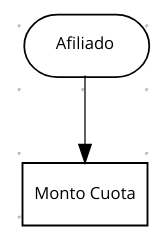
\includegraphics[width=3cm]{drools_diagram.png}
	\end{figure}
\end{center}

\begin{center}
	\begin{figure}
		\includegraphics*[viewport=0 550 789 1175, width=1.3\textwidth]{drools_table.png}
		\includegraphics*[viewport=0 0 789 550, width=1.3\textwidth]{drools_table.png}
	\end{figure}
\end{center}

\paragraph{Gestión de reglas.}
Drools provee un editor visual para la edición de reglas que utilizan \acrshort{dmn}. El editor es una librería web autocontenida, también existe una extensión para Visual Studio Code, que expone la funcionalidad de la misma.

\paragraph{Integración.}
Las reglas de Drools pueden hacer uso de \acrcomplete{pojo}, es decir objetos con campos, getters, setters y constructores, funcionalidad que no pudo ser utilizada en el ejemplo por los problemas mencionados en \cref{para:drools_mantenimiento}.

Alternativamente, los tipos pueden ser definidos utilizando en el editor visual, pasando luego mapas con los valores correspondientes, siendo las claves los nombres de los campos.

\paragraph{Mantenimiento.}\label{para:drools_mantenimiento}
Este motor de reglas es open source y de uso libre, y su desarrollo continúa actualmente activo (hasta la última fecha de edición de esta sección, 20/03/25, la última versión fue publicada el 28/04/24).

Utilizando Ubuntu 22.04.5 LTS, tanto en la extensión como la librería web, se notaron problemas a la hora de importar de otros modelos o de clases Java. Los archivos \verb|.dmn| no eran encontrados por la extensión, mientras que la opción para importar clases Java no estaba disponible. Por otro lado, al cambiar los tipos de las expresiones (Feel Expresion en el ejemplo arriba) al finalizar la edición de uno, los otros volvía a tener el valor inicial de <Undefined>, que es la razón de que tengan ese valor en el ejemplo anterior.

Adicionalmente, incluyendo la librería en un sitio web, únicamente instanciando el componente editor de la librería resulta en numerosos mensajes de advertencia en la consola.

\section{\href{https://openl-tablets.org/}{OpenL Tablets}}
OpenL Tablets es un sistema de gestión de reglas y un motor de reglas basado en la representación de reglas como tablas, desarrollado por el \href{https://openl-tablets.org/community/team}{equipo de OpenL}. Su desarrollo comenzó en 2003 como un projecto interno y fue luego publicado en 2006 en SourceForge. En un principio era únicamente un motor de reglas, convirtiendose en un sistema de gestión de reglas a partir de la versión 5.

\paragraph{Expresividad.}
Para la definición de las reglas se utilizan tablas basadas en Microsoft Excel. Dentro de estas celdas pueden haver valores, acciones o expressiones. Las últimas dos hacen uso de BEX, que es una extensión de la gramática de Java.

\begin{table}[!ht]
	\makeatletter\@ifundefined{tablewidth}{\newlength{\tablewidth}}{}
\makeatother\setlength{\tablewidth}{\dimexpr \textwidth - 3\arrayrulewidth - 6\tabcolsep \relax}
\setlength{\extrarowheight}{-5pt}

\begin{tabular}{|p{0.21\tablewidth}|p{0.27\tablewidth}|p{0.51\tablewidth}|}
		\hline
		\multicolumn{3}{|C{{\dimexpr 1.0\tablewidth + 2\arrayrulewidth + 4\tabcolsep \relax}}|}{\color[HTML]{FFFFFF}\cellcolor[HTML]{000000}Rules Double CalcularCuota(AfiliacionWrapper afiliado)} \\ \hline
		\color[HTML]{000000}\cellcolor[HTML]{CCFFFF}C1
		 & \color[HTML]{000000}\cellcolor[HTML]{CCFFFF}C2
		 & \color[HTML]{000000}\cellcolor[HTML]{CCFFFF}RET1                                                                                                                                         \\ \hline
		\color[HTML]{000000}\cellcolor[HTML]{CCFFFF}categoria
		 & \color[HTML]{000000}\cellcolor[HTML]{CCFFFF}subcategoria
		 & \color[HTML]{000000}\cellcolor[HTML]{CCFFFF}value                                                                                                                                        \\ \hline
		\cellcolor[HTML]{CCFFFF}
		 & \cellcolor[HTML]{CCFFFF}
		 & \color[HTML]{000000}\cellcolor[HTML]{CCFFFF}Double value                                                                                                                                 \\ \hline
		\color[HTML]{000000}\cellcolor[HTML]{FFFF99}Categoria
		 & \color[HTML]{000000}\cellcolor[HTML]{FFFF99}Sub Categoria
		 & \color[HTML]{000000}\cellcolor[HTML]{FFCC99}Fee Value                                                                                                                                    \\ \hline
		\cellcolor[HTML]{FFFF99}
		 & \color[HTML]{000000}\cellcolor[HTML]{FFFF99}CONYUGE
		 & \color[HTML]{000000}\cellcolor[HTML]{FFCC99}=CalcularCuota(conyuge) * 0.7\strut                                                                                                          \\\cline{2-3} \noalign{\vskip 0.5pt}
		\multirow{-2}{0.21\tablewidth}{\color[HTML]{000000}\cellcolor[HTML]{FFFF99}FAMILIAR}
		 & \color[HTML]{000000}\cellcolor[HTML]{FFFF99}DESCENDIENTE\allowbreak\_PRIMER\allowbreak\_GRADO
		 & \color[HTML]{000000}\cellcolor[HTML]{FFCC99}0                                                                                                                                            \\ \hline
		\cellcolor[HTML]{FFFF99}
		 & \color[HTML]{000000}\cellcolor[HTML]{FFFF99}BECARIO
		 & \color[HTML]{000000}\cellcolor[HTML]{FFCC99}=CMMU * ModificadorBecario(afiliado)\strut                                                                                                   \\\cline{2-3} \noalign{\vskip 0.5pt}
		\multirow{-2}{0.21\tablewidth}{\color[HTML]{000000}\cellcolor[HTML]{FFFF99}VOLUNTARIO\allowbreak\_ADHERENTE}
		 & \color[HTML]{000000}\cellcolor[HTML]{FFFF99}AGENTE\allowbreak\_UNSL\allowbreak\_CON\allowbreak\_LICENCIA
		 & \color[HTML]{000000}\cellcolor[HTML]{FFCC99}=afiliado.getHaberPercibido() * ModificadorAgente(afiliado)                                                                                  \\ \hline
		\cellcolor[HTML]{FFFF99}
		 & \cellcolor[HTML]{FFFF99}
		 & \color[HTML]{000000}\cellcolor[HTML]{FFCC99}=error(``categoria desconocida'')                                                                                                            \\ \hline
	\end{tabular}

	\caption{Tabla principal del ejemplo}
\end{table}

\begin{table}[!ht]
	\makeatletter\@ifundefined{tablewidth}{\newlength{\tablewidth}}{}
\makeatother\setlength{\tablewidth}{\dimexpr \textwidth - 2\arrayrulewidth - 4\tabcolsep \relax}
\setlength{\extrarowheight}{-5pt}

\begin{tabular}{|p{0.33\tablewidth}|p{0.67\tablewidth}|}
	\hline
	\multicolumn{2}{|C{{\dimexpr 1.0\tablewidth + 1\arrayrulewidth + 2\tabcolsep \relax}}|}{\color[HTML]{FFFFFF}\cellcolor[HTML]{000000}Environment} \\ \hline
	\color[HTML]{000000}\cellcolor[HTML]{FFFF99}import
	 & \color[HTML]{000000}\cellcolor[HTML]{FFFF99}com.example.afiliacion\allowbreak\_wrapper                                                        \\ \hline
\end{tabular}

	\caption{Importación de las clases de Java}
	\label{tab:openl_java_import}
\end{table}

\begin{table}[!ht]
	\makeatletter\@ifundefined{tablewidth}{\newlength{\tablewidth}}{}
\makeatother\setlength{\tablewidth}{\dimexpr \textwidth - 3\arrayrulewidth - 6\tabcolsep \relax}
\setlength{\extrarowheight}{-5pt}

\begin{tabular}{|p{0.28\tablewidth}|p{0.25\tablewidth}|p{0.47\tablewidth}|}
	\hline
	\multicolumn{3}{|C{{\dimexpr 1.0\tablewidth + 2\arrayrulewidth + 4\tabcolsep \relax}}|}{\color[HTML]{FFFFFF}\cellcolor[HTML]{000000}Rules Double ModificadorBecario(AfiliacionWrapper afiliado)} \\ \hline
	\multicolumn{2}{|C{{\dimexpr 0.5330525030525031\tablewidth + 1\arrayrulewidth + 2\tabcolsep \relax}}|}{\color[HTML]{000000}\cellcolor[HTML]{CCFFFF}C3}
	 & \color[HTML]{000000}\cellcolor[HTML]{CCFFFF}RET1                                                                                                                                              \\ \hline
	\multicolumn{2}{|C{{\dimexpr 0.5330525030525031\tablewidth + 1\arrayrulewidth + 2\tabcolsep \relax}}|}{\color[HTML]{000000}\cellcolor[HTML]{CCFFFF}edad}
	 & \color[HTML]{000000}\cellcolor[HTML]{CCFFFF}value                                                                                                                                             \\ \hline
	\color[HTML]{000000}\cellcolor[HTML]{CCFFFF}int min
	 & \color[HTML]{000000}\cellcolor[HTML]{CCFFFF}int max
	 & \color[HTML]{000000}\cellcolor[HTML]{CCFFFF}Double value                                                                                                                                      \\ \hline
	\color[HTML]{000000}\cellcolor[HTML]{FFFF99}Desde
	 & \color[HTML]{000000}\cellcolor[HTML]{FFFF99}Hasta
	 & \color[HTML]{000000}\cellcolor[HTML]{FFCC99}Modificador                                                                                                                                       \\ \hline
	\cellcolor[HTML]{FFFF99}
	 & \color[HTML]{000000}\cellcolor[HTML]{FFFF99}30
	 & \color[HTML]{000000}\cellcolor[HTML]{FFCC99}0.45                                                                                                                                              \\ \hline
	\color[HTML]{000000}\cellcolor[HTML]{FFFF99}31
	 & \color[HTML]{000000}\cellcolor[HTML]{FFFF99}45
	 & \color[HTML]{000000}\cellcolor[HTML]{FFCC99}0.82                                                                                                                                              \\ \hline
	\color[HTML]{000000}\cellcolor[HTML]{FFFF99}46
	 & \color[HTML]{000000}\cellcolor[HTML]{FFFF99}55
	 & \color[HTML]{000000}\cellcolor[HTML]{FFCC99}1                                                                                                                                                 \\ \hline
	\color[HTML]{000000}\cellcolor[HTML]{FFFF99}56
	 & \color[HTML]{000000}\cellcolor[HTML]{FFFF99}65
	 & \color[HTML]{000000}\cellcolor[HTML]{FFCC99}1.2                                                                                                                                               \\ \hline
	\color[HTML]{000000}\cellcolor[HTML]{FFFF99}66
	 & \cellcolor[HTML]{FFFF99}
	 & \color[HTML]{000000}\cellcolor[HTML]{FFCC99}2                                                                                                                                                 \\ \hline
\end{tabular}

	\caption{Tabla modificador becario}
\end{table}

\begin{table}[!ht]
	\makeatletter\@ifundefined{tablewidth}{\newlength{\tablewidth}}{}
\makeatother\setlength{\tablewidth}{\dimexpr \textwidth - 3\arrayrulewidth - 6\tabcolsep \relax}
\setlength{\extrarowheight}{-5pt}

\begin{tabular}{|p{0.23\tablewidth}|p{0.24\tablewidth}|p{0.53\tablewidth}|}
	\hline
	\multicolumn{3}{|C{{\dimexpr 0.9999999999999999\tablewidth + 2\arrayrulewidth + 4\tabcolsep \relax}}|}{\color[HTML]{FFFFFF}\cellcolor[HTML]{000000}Rules Double ModificadorAgente(AfiliacionWrapper afiliado)} \\ \hline
	\multicolumn{2}{|C{{\dimexpr 0.4692429792429792\tablewidth + 1\arrayrulewidth + 2\tabcolsep \relax}}|}{\color[HTML]{000000}\cellcolor[HTML]{CCFFFF}C3}
	 & \color[HTML]{000000}\cellcolor[HTML]{CCFFFF}RET1                                                                                                                                                            \\ \hline
	\multicolumn{2}{|C{{\dimexpr 0.4692429792429792\tablewidth + 1\arrayrulewidth + 2\tabcolsep \relax}}|}{\color[HTML]{000000}\cellcolor[HTML]{CCFFFF}edad}
	 & \color[HTML]{000000}\cellcolor[HTML]{CCFFFF}value                                                                                                                                                           \\ \hline
	\color[HTML]{000000}\cellcolor[HTML]{CCFFFF}int min
	 & \color[HTML]{000000}\cellcolor[HTML]{CCFFFF}int max
	 & \color[HTML]{000000}\cellcolor[HTML]{CCFFFF}Double value                                                                                                                                                    \\ \hline
	\color[HTML]{000000}\cellcolor[HTML]{FFFF99}Desde
	 & \color[HTML]{000000}\cellcolor[HTML]{FFFF99}Hasta
	 & \color[HTML]{000000}\cellcolor[HTML]{FFCC99}Modificador                                                                                                                                                     \\ \hline
	\cellcolor[HTML]{FFFF99}
	 & \color[HTML]{000000}\cellcolor[HTML]{FFFF99}30
	 & \color[HTML]{000000}\cellcolor[HTML]{FFCC99}0.4                                                                                                                                                             \\ \hline
	\color[HTML]{000000}\cellcolor[HTML]{FFFF99}31
	 & \color[HTML]{000000}\cellcolor[HTML]{FFFF99}45
	 & \color[HTML]{000000}\cellcolor[HTML]{FFCC99}0.78                                                                                                                                                            \\ \hline
	\color[HTML]{000000}\cellcolor[HTML]{FFFF99}46
	 & \color[HTML]{000000}\cellcolor[HTML]{FFFF99}55
	 & \color[HTML]{000000}\cellcolor[HTML]{FFCC99}0.95                                                                                                                                                            \\ \hline
	\color[HTML]{000000}\cellcolor[HTML]{FFFF99}56
	 & \color[HTML]{000000}\cellcolor[HTML]{FFFF99}65
	 & \color[HTML]{000000}\cellcolor[HTML]{FFCC99}1.13                                                                                                                                                            \\ \hline
	\color[HTML]{000000}\cellcolor[HTML]{FFFF99}66
	 & \cellcolor[HTML]{FFFF99}
	 & \color[HTML]{000000}\cellcolor[HTML]{FFCC99}1.86                                                                                                                                                            \\ \hline
\end{tabular}

	\caption{Tabla secundaria modificador agente UNSL}
\end{table}

\paragraph{Gestión de reglas.}
El motor posee una aplicación web para la creación, modificación, eliminación, prueba y versionado. Además, se separan los repositorios de diseño y producción, permitiendo la colaboración en edición de reglas y el versionado de las mismas de forma independiente del \acrshort{si}. Alternativamente, pueden utilizarse Microsoft Excel, of software similar como Libre Office, para la creación, modificación y eliminación de las reglas.

\paragraph{Integración.}
Por otra parte, OpenL Tablets posee otra aplicación para exponer las reglas almacenadas en un repositorio como servicios web. Alternativamente, brinda clases de utilidad para la compilación de las reglas. Estas utilizan las tablas para generar clases wrapper, las cuales también pueden ser específicadas manualmente. En caso de utilzar las clases generadas, las reglas pueden accederse por medio de la reflección, siendo métodos de las clases con los mismos nombres de las reglas.

Las reglas de OpenL pueden hacer uso directo de las instancias de las clases Java. Para esto, se utiliza una tabla para importar las mismas, como la presente en \cref{tab:openl_java_import}.

\paragraph{Mantenimiento.}
Este motor de reglas es open source y de uso libre, y su desarrollo continúa actualmente activo (hasta la última fecha de edición de esta sección, 20/03/25, la última versión fue publicada el 28/02/2025).

